% !TeX root = ../main.tex

\chapter{基于模型集成的筛选规划算法}

\section{条件风险价值CVaR}

虽然目前最先进的基于模型的方法已经取得了显著的性能,但它们通常只适合于训练的环境,当部署到扰动的真实环境时,性能往往会急剧下降。条件风险价值(CVaR)是一种用于计算最大风险的指标,借由CVaR指标,我们可以通过学习消极样本数据来提高强化学习算法的鲁棒性,得以解决强化学习算法中安全性不足的一大挑战。

\begin{figure}
  \centering
  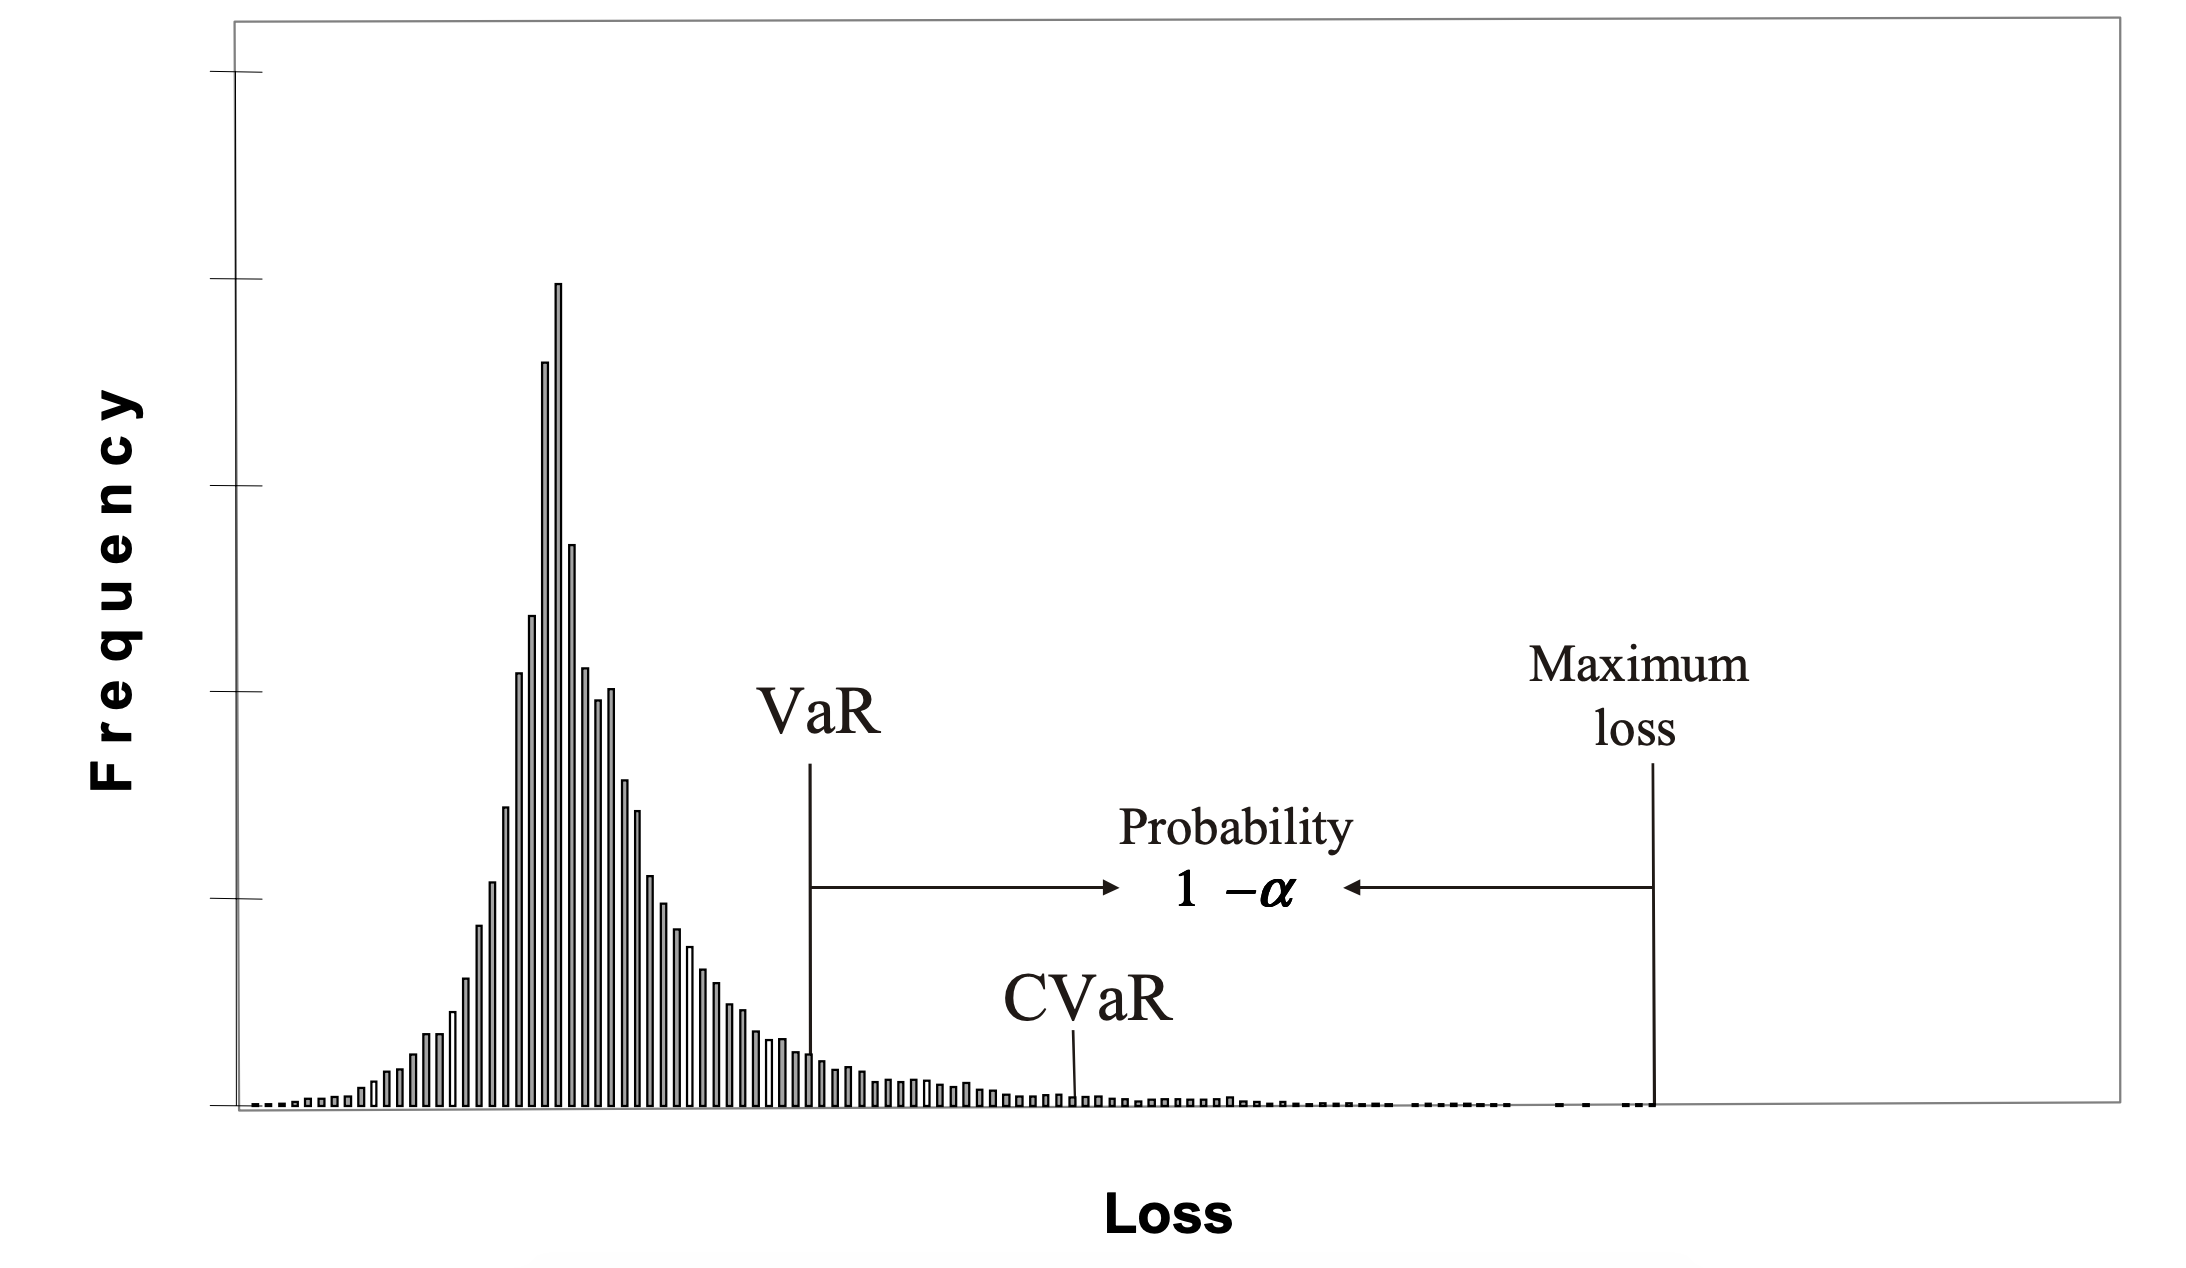
\includegraphics[width=\linewidth]{figures/CVaR.png}
  \caption{CVaR计算示意图}
  \label{fig:cvar}
\end{figure}

如图\ref{fig:cvar}所示,首先定义风险价值(VaR):
\begin{equation}
    \mathrm{VaR}_\alpha=\inf\left\{z\mid\mathrm{P}(Z\geq z)\leq 1-\alpha\right\}
\end{equation}
VaR的含义为在给定置信度$\alpha$下的最大可能损失,更进一步地,我们可定义条件风险价值(CVaR):
\begin{equation}
    \mathrm{CVaR}_\alpha = \mathbb{E}\left[Z\mid Z\geq \mathrm{VaR}_\alpha\right]
\end{equation}
CVaR的含义为收益风险超过VaR部分的平均期望损失。

基于CVaR的思想,我们可以类似的在强化学习经验回放样本池中加入这一设计,将更低奖励反馈的样本加以更多的学习,而对过高奖励反馈的样本进行适当的筛选和丢弃,确保强化学习算法所学策略能够更稳定地处理高风险状态。

\section{MBDP算法设计}

正如前一节的介绍,尽管在CVaR条件风险价值的思路下可以实现鲁棒性的提升,但是显然易见的是筛选丢弃样本的做法会损失一部分性能。为此,我们提出了基于模型集成的筛选规划算法(Model-Based Dropout Planning,MBDP),在做到提升算法鲁棒性的同时维持原有的算法性能。

\subsection{环境模型的集成学习与筛选}\label{sec:model-method}

传统的不确定性环境建模和集成方法,虽然已经能够较好地模拟真实复杂环境并且捕捉到环境的不确定性 \cite{duan2007multi},但并不能很好地控制模拟的精准程度,本论文在不确定性环境建模的基础上,结合传统集成学习的方法,设计了模型的集成和筛选机制。

具体地,首先训练学习一组环境模型集合$\{\mathcal{M}_{\phi_1},\mathcal{M}_{\phi_2},\ldots\}$,集合中每一个环境模型都是一个概率神经网络,其输出$\mu_{\phi_i},\sigma_{\phi_i}$构成高斯分布$\mathcal{N}(\mu_{\phi_i}(s,a),\sigma_{\phi_i}(s,a))$,环境模型对于下一时刻的状态预测则服从该分布,即

\begin{equation}
    s^\prime \sim \mathcal{M}_{\phi_i}(s,a) = \mathcal{N}(\mu_{\phi_i}(s,a),\sigma_{\phi_i}(s,a))
\end{equation}

在训练环境模型的同时,根据真实环境中采样得到的真实样本$(S,A)$,可以计算并记录模型的期望偏差:
\begin{equation}
    \mathrm{bias}(\phi_i) = \underset{S,A\sim \pi,\mathcal{P}}{\mathbb{E}}\|\mathcal{M}_{\phi_i}(S,A)-\mathcal{P}(S,A)\|
\end{equation}

其中$\|\cdot\|$是状态空间$\mathcal{S}$上的范数距离,该式的含义为所训练的环境模型$\mathcal{M}$与真实环境$\mathcal{P}$之间的范数意义距离。在上述模型集合的基础上,首先根据所计算的$\mathrm{bias}(\phi_i)$大小进行升序重排,并设定一个概率参数$\alpha\in(0,1]$,筛选出$\mathrm{bias}$在$\alpha$分位数以前的模型,保留得到筛选后的模型集合$\mathcal{M}^\alpha = \{\mathcal{M}_{\phi_1},\mathcal{M}_{\phi_2},\ldots,\mathcal{M}_{\phi_{N_\alpha}}\}$,其中$N_\alpha$是前面所描述的升序排序后的集合索引$\left\{1,2,\ldots,N_\alpha,\ldots\right\}$中的$\alpha$分位数。

需要注意的是,用于集成的不确定性模型集合并不是$\mathrm{bias}$越小越好,过小的$\mathrm{bias}$可能意味着过拟合的环境模型。参数$\alpha$的重要用处是可以动态地调整模型集合的整体精确性,它能与下一节将介绍的参数$\beta$协作调整强化学习的收益性能与鲁棒性。

\subsection{环境模型的数据生成与筛选}\label{sec:rollout-method}

传统的基于模型的强化学习算法在得到环境模型后,往往是以期望收益为目标进行最大化优化,但是期望意义下的最优并不意味着在任意环境下都能有优秀的表现,在实际部署策略的时候,当面临一些受干扰的信息不足的状态,策略容易做出一些不合理甚至危险的决策,导致强化学习在实际部署中不稳定。

为了解决这一问题,本论文提出了一种主动关注较坏情况的样本筛选机制,适当延缓强化学习训练速度,提升决策策略的鲁棒性。

具体地,基于上一节得到的$\mathcal{M}^{\alpha}$模型集合,在每一步都随机抽取一个模型$\mathcal{M}_{\phi_i}\in\mathcal{M}^\alpha$,然后使用该模型进行下一时刻的状态预测,即$s_{t+1}\sim \mathcal{M}_{\phi_t}(s_t,a_t), \phi_t\in\Phi_\alpha$,这样的一组状态和动作组成模拟样本$x=\left(s_{t+1},s_t,a_t\right)$,填入缓存池,然后相似地以一个概率参数$\beta\in(0,1]$进行筛选,从中挑选出反馈奖励值相对较低的样本,得到一个筛选后的$\beta$分位数样本集合

\begin{equation}
    \mathcal{B}_\beta^{\pi,\mathcal{M}^\alpha}=\left\{x|x\in\mathcal{B}^{\pi,\mathcal{M}^\alpha},r(x)\leq r_\beta(\mathcal{B}^{\pi,\mathcal{M}^\alpha})\right\}
\end{equation}
其中$\mathcal{B}^{\pi,\mathcal{M}^\alpha}=\left\{x|x\triangleq\left(s_{t+1},s_t,a_t\right)\sim\pi,\mathcal{M}^\alpha\right\}$, $r_\beta(\mathcal{B}^{\pi,\mathcal{M}^\alpha})$ 是缓存池 $\mathcal{B}^{\pi,\mathcal{M}^\alpha}$的$\beta$分位数。

\subsection{算法描述与整体框架}

\begin{figure}[tbh]
\centering
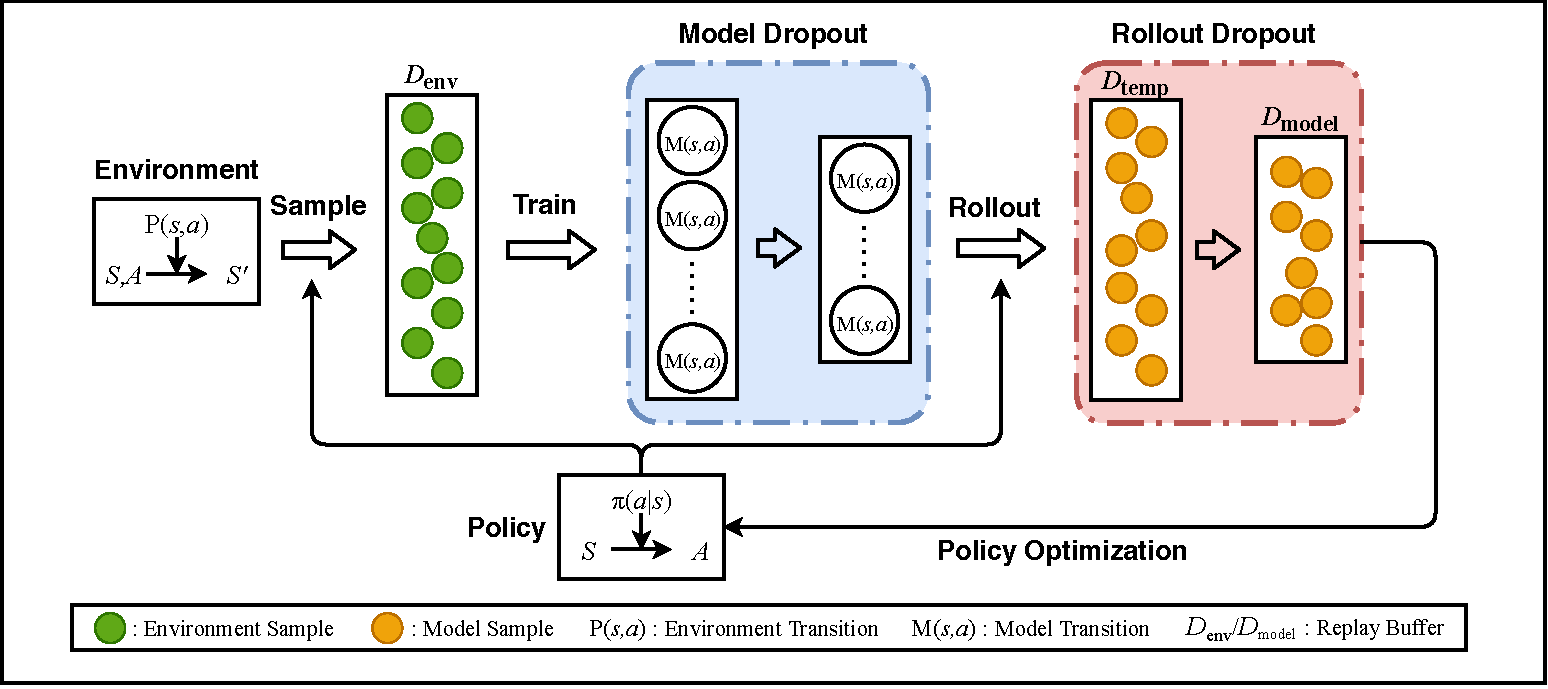
\includegraphics[width=\textwidth]{figures/mbdp.pdf}
\caption{算法整体框架结构。}
\label{fig:algo-structure}
\end{figure}

由于在强化学习中模拟误差越小,算法的收敛性能则越好,观察公式(\ref{eq:MBDP-bound})中的误差上界$D_{\alpha,\beta}(\mathcal{M})$可知,强化学习的算法性能与参数$\alpha$成反比,与参数$\beta$成正比,又根据\ref{sec:model-method}节和\ref{sec:rollout-method}节的介绍可知,策略的鲁棒性显然与参数$\alpha$成正比,与参数$\beta$成反比,恰好与前面的作用效果相反。

因此,本论文可以动态性地调整参数$\alpha,\beta$来取得算法性能和最终策略鲁棒性之间的平衡,从而得到不同属性的强化学习决策策略:

\begin{itemize}
    \item \textbf{平衡的决策策略}:将参数$\alpha$和$\beta$调整为适中大小的概率值,适用于一般的普通环境;
    \item \textbf{收益性能较高的决策策略}:将参数$\alpha$调整为较小的概率值,$\beta$调整为较大的概率值,适用于相对稳定的环境;
    \item \textbf{鲁棒性较好的决策策略}:将参数$\alpha$调整为较大的概率值,$\beta$调整为较小的概率值,适用于干扰较大的环境。
\end{itemize}

基于\ref{sec:model-method}节和\ref{sec:rollout-method}节的提出的改进方案思路,将其整合进传统的基于模型的强化学习算法框架,得到改进的算法,算法整体框架如图\ref{fig:algo-structure}所示。

首先通过与环境交互产生样本,用于训练概率模型并集成模拟,两个筛选模块作为主要改进加入到模拟数据生成的环节中,最终提供给策略优化公式对策略$\pi(a|s)$进行优化,并进行下一轮迭代。MBDP算法的主要流程如算法~\ref{algo:our-method}所示。

\begin{algorithm}[tb]
\caption{基于模型集成的筛选规划算法 (\textbf{MBDP})}
\label{algo:our-method}
\begin{algorithmic}
\STATE 初始化超参数、策略 $\pi_\theta$、环境经验回放池 $\mathcal{D}_{\mathrm{env}}$、模型经验回放池 $\mathcal{D}_{\mathrm{model}}$\\
\FOR{$N_\mathrm{epoch}$ 迭代次数}
    \STATE 在环境中使用决策策略 $\pi_\theta$采取行动动作
    \STATE 将样本加入 $\mathcal{D}_{\mathrm{env}}$\\
    \FOR{$N_\mathrm{train}$ 迭代次数}
        \STATE  在收集的数据集$\mathcal{D}_{\mathrm{env}}$上训练概率模型$\mathcal{M}$\\
        \STATE 根据模型偏差$\mathrm{bias}({\phi_i})$构建模型子集 $\mathcal{M}^\beta = \{\mathcal{M}_{\phi_1},\ldots,\mathcal{M}_{\phi_{N_{1-\beta}}}\}$\\
        \FOR{$t=1,2,\ldots ,T$}
            \STATE 从 $\mathcal{M}^\beta$ 中随机抽选模型$\mathcal{M}_{\phi_t}$\\
            \STATE 在模型$\mathcal{M}_{\phi_t}$ 上使用策略$\pi_\theta$,生成样本$x=\left(s_{t+1},s_t,a_t\right)$ \\
            \STATE 将样本填入缓存回放池 $\mathcal{B}^{\pi,\mathcal{M}^\beta}$\\
        \ENDFOR
        \STATE 根据状态$s, \forall s\in\mathcal{S}$分组后计算$100\times(1-\alpha)$分位数,得到 $r_{1-\alpha}(\mathcal{B}^{\pi,\mathcal{M}^\beta}|s)$\\
        \FOR{$x\in \mathcal{B}^{\pi,\mathcal{M}^\beta}$}
            \IF{$r(x)\leq r_{1-\alpha}(\mathcal{B}^{\pi,\mathcal{M}^\beta}|s_t)$}
                \STATE 将 $x$ 填入 $\mathcal{D}_{\mathrm{model}}$
            \ENDIF
        \ENDFOR
    \ENDFOR
    \STATE 在$\mathcal{D}_{\mathrm{model}}$上优化$\pi_\theta$: $\theta\leftarrow \theta - \lambda\nabla_\theta J_\theta(\mathcal{D}_{\mathrm{model}})$
\ENDFOR
\end{algorithmic}
\end{algorithm}

\section{算法理论分析}

在MBDP方法中,缓存池里的模拟样本构成的期望收益记为${V}^{\pi,\mathcal{M}^\alpha}_\beta$。本论文可以证明,加入样本筛选机制后的模拟期望收益,与真实环境中期望收益的差异为一个受参数$\beta$控制的上界,如定理 \ref{the:beta-drop-bound} 所述。

\begin{theorem}\label{the:beta-drop-bound}

记$R_{m}$为奖励函数$r(s,a)$的上确界, 即 $R_{m}=\underset{s\in\mathcal{S},a\in\mathcal{A}}{\sup}r(s,a)$,在环境模型$\mathcal{M}_\phi$上使用样本筛选机制后,所得期望收益与真实环境中期望收益的差异值存在误差上界:

\begin{equation}
    |{V}_\alpha^{\pi, \mathcal{M}_{\phi}} - {V}^{\pi,\mathcal{M}_{\phi}}| \leq \frac{\alpha(1+\alpha)}{(1-\alpha)(1-\gamma)}\mathrm{R_{m}} \triangleq \epsilon_\alpha
\label{eq:eps-beta}
\end{equation}

\end{theorem}

定理~\ref{the:beta-drop-bound}的重要意义是,即使筛选掉一批模拟样本,环境模型给出的模拟数据仍具备一定的可靠性,该可靠性由概率参数$\alpha$控制。该定理的证明如下。

\begin{proof}


首先可以证明,对于两个不相交的集合 $A$ 和 $B$($A\cap B=\varnothing$) ,满足下列关系式

\begin{equation}
    \mathbb{E}_{A\cup B}[X] = \mathbb{E}_A[X]\mathrm{P}(A)+\mathbb{E}_B[X]\mathrm{P}(B)
\end{equation}

基于上述性质,可以计算得到

\begin{align*}
    &\mathbb{E}\left[{\sum}_{s_0\in\mathcal{S},\{a_0,s_1,\ldots\} \sim\pi,\mathcal{M}_\phi}\left[\gamma^t r(s_t,a_t)\right]\right] \\
    &= (1-\alpha)\cdot \mathbb{E}\left[{\sum}_{\{s_0,a_0,\ldots\} \sim\mathcal{B}_\alpha^{\pi,\mathcal{M}_\phi}}\left[\gamma^t r(s_t,a_t)\right]\right] + \alpha\cdot\mathbb{E}\left[{\sum}_{\{s_0,a_0,\ldots\} \not\sim\mathcal{B}_\alpha^{\pi,\mathcal{M}_\phi}}\left[\gamma^t r(s_t,a_t)\right]\right]
\end{align*}

根据定义 (\ref{def:eta-s}), (\ref{def:eta-expectation}) 和 (\ref{def:eta-beta}),我们可以得到

\begin{align}
{V}^{\pi,\mathcal{M}_\phi}_\alpha&=\mathbb{E}\left[{\sum}_{\{s_0,a_0,\ldots\} \sim\mathcal{B}_\alpha^{\pi,\mathcal{M}_\phi}}\left[\gamma^t r(s_t,a_t)\right]\right]\notag\\
&=\frac{1}{1-\alpha}\mathbb{E}\left[{\sum}_{s_0\in\mathcal{S},\{a_0,s_1,\ldots\} \sim\pi,\mathcal{M}_\phi}\left[\gamma^t r(s_t,a_t)\right]\right]-\frac{\alpha}{1-\alpha}\mathbb{E}\left[{\sum}_{\{s_0,a_0,\ldots\} \not\sim\mathcal{B}_\alpha^{\pi,\mathcal{M}_\phi}}\left[\gamma^t r(s_t,a_t)\right]\right]\notag\\
&=\frac{1}{1-\alpha}\underset{s\in{\mathcal{S}}}{\mathbb{E}}\left[{V}^{\pi,\mathcal{M}_\phi}(s)\right]-\frac{\alpha}{1-\alpha}\mathbb{E}\left[{\sum}_{\tau \not\sim\mathcal{B}_\alpha^{\pi,\mathcal{M}_\phi}}\left[\gamma^t r(s_t,a_t)\right]\right]\notag\\
&=\frac{1}{1-\alpha}{V}^{\pi,\mathcal{M}_\phi}-\frac{\alpha}{1-\alpha}\mathbb{E}\left[{\sum}_{\tau \not\sim\mathcal{B}_\alpha^{\pi,\mathcal{M}_\phi}}\left[\gamma^t r(s_t,a_t)\right]\right]\label{proof:lem42p1}
\end{align}
其中 $\tau\triangleq\{s_0,a_0,\ldots\}$。根据定义 (\ref{def:batch-alpha-beta}) 以及  $\mathrm{R}_{m}=\underset{s\in\mathcal{S},a\in\mathcal{A}}{\sup}r(s,a)$,可得

\begin{align*}
\mathbb{E}\left[{\sum}_{\tau \not\sim\mathcal{B}_\alpha^{\pi,\mathcal{M}_\phi}}\left[\gamma^t r(s_t,a_t)\right]\right] &\leq\int_{\tau\not\sim{\mathcal{B}_\alpha^{\pi,\mathcal{M}_\phi}}}\left[\sum_{t=0}^\infty\gamma^t \mathrm{R}_m\right]p(\tau)\mathrm{d}\tau\\
&=\left[\sum_{t=0}^\infty\gamma^t\right]\mathrm{R}_m\int_{\tau\not\sim{\mathcal{B}_\alpha^{\pi,\mathcal{M}_\phi}}}p(\tau)\mathrm{d}\tau\\
&= \frac{1}{1-\gamma}\mathrm{R}_m \int_{\tau\not\sim{\mathcal{B}_\alpha^{\pi,\mathcal{M}_\phi}}}p(\tau)\mathrm{d}\tau\\
&=\frac{\alpha}{1-\gamma}\mathrm{R}_m \tag{By definition of $\mathcal{B}_\alpha^{\pi,\mathcal{M}_\phi}$}\\
\end{align*}

与之相似地,我们可以得到

\begin{align*}
V^{\pi,\mathcal{M}_\phi} = \mathbb{E}\left[{\sum}_{\tau \sim\mathcal{B}^{\pi,\mathcal{M}_\phi}}\left[\gamma^t r(s_t,a_t)\right]\right] &\leq\int_{\tau \sim\mathcal{B}^{\pi,\mathcal{M}_\phi}}\left[\sum_{t=0}^\infty\gamma^t \mathrm{R}_m\right]p(\tau)\mathrm{d}\tau\\
&=\left[\sum_{t=0}^\infty\gamma^t\right]\mathrm{R}_m\int_{\tau \sim\mathcal{B}^{\pi,\mathcal{M}_\phi}}p(\tau)\mathrm{d}\tau\\
&= \frac{1}{1-\gamma}\mathrm{R}_m \int_{\tau \sim\mathcal{B}^{\pi,\mathcal{M}_\phi}}p(\tau)\mathrm{d}\tau\\
&=\frac{1}{1-\gamma}\mathrm{R}_m\\
\end{align*}

根据上述推导得到的两个不等式关系以及方程式 (\ref{proof:lem42p1}),可知

\begin{align}
|{V}_\alpha^{\pi, \mathcal{M}_{\phi}} - {V}^{\pi,\mathcal{M}_{\phi}}| &=  \left|\frac{\alpha}{1-\alpha}V^{\pi,\mathcal{M}_\phi}-\frac{\alpha}{1-\alpha}\mathbb{E}\left[{\sum}_{\tau \not\sim\mathcal{B}_\alpha^{\pi,\mathcal{M}_\phi}}\left[\gamma^t r(s_t,a_t)\right]\right]\right| \notag\\
&\leq\frac{\alpha}{1-\alpha}\left(\left|V^{\pi,\mathcal{M}_\phi}\right|+\left|\mathbb{E}\left[{\sum}_{\tau \not\sim\mathcal{B}_\alpha^{\pi,\mathcal{M}_\phi}}\left[\gamma^t r(s_t,a_t)\right]\right]\right|\right)\notag\\
&\leq \frac{\alpha}{1-\alpha}\left(\frac{1}{1-\gamma}\mathrm{R}_m+\frac{\alpha}{1-\gamma}\mathrm{R}_m\right) \notag\\
&=\frac{\alpha(1+\alpha)}{(1-\alpha)(1-\gamma)}\mathrm{R_{m}} \label{eq:lem42}
\end{align}

\end{proof}

更进一步地,我们可以证明在同时加入模拟数据筛选模块和集成模型筛选模块后,所得到的策略期望价值仍然与真实环境下的策略收益存在一个可控的误差上界,并且该上界由筛选比例$\alpha$和$\beta$控制。

\begin{theorem}\label{the:MBDP-bound}

设 $K\geq 0$ 是一项常数。 在同时加入模拟数据筛选模块和集成模型筛选模块后所得到的策略期望价值 ${V}_\alpha^{\pi, \mathcal{M}^\beta}$,与真实环境$\mathcal{P}$下所能得到的期望策略价值 ${V}^{\pi, \mathcal{P}}$存在一个误差上界:
\begin{equation}
\left|{V}_\alpha^{\pi, \mathcal{M}^\beta}-{V}^{\pi, \mathcal{P}}\right|\leq D_{\alpha,\beta}(\mathcal{M})
\end{equation}
其中
\begin{equation}\label{eq:MBDP-bound}
D_{\alpha,\beta}(\mathcal{M})\triangleq\frac{(1-\beta)\gamma K}{1-\gamma}\epsilon_{\mathcal{M}}+\frac{\alpha(1+\alpha)(1-\beta)}{(1-\alpha)(1-\gamma)}\mathrm{R}_m
\end{equation}
并且
\begin{equation}\label{def:delta-M}
\epsilon_{\mathcal{M}}\triangleq\underset{\phi\in\Phi}{\mathbb{E}}\left[\underset{s,a\sim \pi,\mathcal{P}}{\mathbb{E}}\left[\left\|\mathcal{M}_\phi(s, a)-\mathcal{P}(s, a)\right\|\right]\right]
\end{equation}

\end{theorem}
为了证明上述定理,我们首先需要引入两个引理

\begin{lemma}\label{lem:proof-for-lem41}

定义

\begin{equation}\label{def:G-sa}
G^{\pi,\mathcal{M}}(s,a)=\underset{\hat{s}'\sim\mathcal{M}(\cdot|s,a)}{\mathbb{E}}{{V}^{\pi,\mathcal{M}}}(\hat{s}') - \underset{s'\sim\mathcal{P}(\cdot|s,a)}{\mathbb{E}}{{V}^{\pi,\mathcal{M}}}(s')
\end{equation}
对于任意策略 $\pi$ 和任意动态模型 $\mathcal{M},\mathcal{M}'$,存在如下关系式

\begin{equation}
{V}^{\pi,\mathcal{M}'} - {V}^{\pi,\mathcal{M}} = \frac{\gamma}{1-\gamma}\underset{S,A\sim\pi,\mathcal{M}}{\mathbb{E}}\left[G^{\pi,\mathcal{M}'}(S,A)\right]
\end{equation}

\end{lemma}

引理 \ref{lem:proof-for-lem41} 引用自Luo等人提出的定理,在其基础上,我们可以进一步推出如下的引理\ref{lem:mb-bound}。

\begin{lemma}\label{lem:mb-bound}
设基于模型方法所能取得的价值函数 ${V}^{\pi,\mathcal{M}}$ 在状态空间$\mathcal{S}$上是Lipschitz连续的,并设$K$为 Lipschitz常数,。记$\mathcal{P}$表示真实环境的状态转移概率分布,则有如下的不等式关系:
\begin{equation}
\left|{V}^{\pi, \mathcal{M}}-{V}^{\pi, \mathcal{P}}\right| \leq\frac{\gamma}{1-\gamma}K\cdot\mathrm{bias}
\end{equation}
其中
\begin{equation}
\mathrm{bias} \triangleq \underset{s,a\sim \pi,\mathcal{P}}{\mathbb{E}}\left\|\mathcal{M}(s, a)-\mathcal{P}(s, a)\right\|
\end{equation}

\label{theo:mb-bound}
\end{lemma}

在引理 \ref{lem:mb-bound}中, 我们假设了关于估计模型$\mathcal{M}$的期望收益${V}^{\pi,\mathcal{M}}(s)$ 关于任意范数距离$\|\cdot\|$都是Lipschitz连续的,即
\begin{equation}\label{assum:lip}
    \left|{V}^{\pi,\mathcal{M}}(s)-{V}^{\pi,\mathcal{M}}(s^{\prime})\right| \leq K\left\|s-s^{\prime}\right\|, \forall s, s^{\prime} \in \mathcal{S}
\end{equation}
其中$K\in \mathbb{R}^+$ 是一个Lipschitz常数。该假设的意义是相近的状态应该拥有相似的价值估计,对于绝大多数场景而言,这一假设显然都是成立的。引理~\ref{lem:mb-bound}的证明如下:

\begin{proof}

根据$G^{\pi,\mathcal{M}}(s,a)$在公式(\ref{def:G-sa})的定义,以及假设 ${V}^{\pi,\mathcal{M}}(s)$ 满足 Lipschitz 连续性(\ref{assum:lip}), 我们可以得到

\begin{equation}\label{eq:G-leq}
|G^{\pi,\mathcal{M}}(s,a)|\leq K\|\mathcal{M}(s,a)-\mathcal{P}(s,a)\|
\end{equation}
可以证明
\begin{align*}
\left|{V}^{\pi, \mathcal{M}}-{V}^{\pi, \mathcal{P}}\right| &= \frac{\gamma}{1-\gamma}\left|\underset{s,a\sim\pi,\mathcal{P}}{\mathbb{E}}\left[G^{\pi,\mathcal{M}}(s,a)\right]\right|\\
&\leq \frac{\gamma}{1-\gamma}\underset{s,a\sim\pi,\mathcal{P}}{\mathbb{E}}\left[\left|G^{\pi,\mathcal{M}}(s,a)\right|\right]\\
&\leq \frac{\gamma}{1-\gamma}\underset{s,a\sim\pi,\mathcal{P}}{\mathbb{E}}K\|\mathcal{M}(s,a)-\mathcal{P}(s,a)\|\\
&= \frac{\gamma}{1-\gamma}K\cdot\underset{s,a\sim\pi,\mathcal{P}}{\mathbb{E}}\|\mathcal{M}(s,a)-\mathcal{P}(s,a)\|\\
&\triangleq \frac{\gamma}{1-\gamma}K\cdot\mathrm{bias}
\end{align*}

\end{proof}

定理~\ref{the:MBDP-bound}的重要意义是,在加入模拟数据筛选模块和集成模型筛选模块后,模型给出的模拟数据与传统的模拟方式相比只存在一个可控的误差上界,对强化学习的训练带来的误差影响并不大,在该可控范围内,如前文对筛选机制的具体描述,本论文能够得到鲁棒性更好的决策策略。基于定理~\ref{the:beta-drop-bound}和引理~\ref{lem:mb-bound},可证明定理\ref{the:MBDP-bound},证明过程如下。

\begin{proof}

根据定理~\ref{the:beta-drop-bound}和引理~\ref{lem:mb-bound},首先可以证明

\begin{align}
\left|{V}_\alpha^{\pi, \mathcal{M}^\beta}-{V}^{\pi, \mathcal{P}}\right|&=\left|\int_{\Phi_\beta}{V}_\alpha^{\pi, \mathcal{M}_{\phi}}p(\phi)\mathrm{d}\phi-{V}^{\pi, \mathcal{P}}\right| \notag\\
&=\left|\int_{\Phi_\beta}\left({V}_\alpha^{\pi, \mathcal{M}_{\phi}}-{V}^{\pi, \mathcal{P}}\right)p(\phi)\mathrm{d}\phi\right| \notag\\
&\leq\int_{\Phi_\beta}\left|{V}_\alpha^{\pi, \mathcal{M}_{\phi}}-{V}^{\pi, \mathcal{P}}\right|p(\phi)\mathrm{d}\phi\\
&\leq\int_{\Phi_\beta}\left(\left|{V}^{\pi, \mathcal{M}_{\phi}}-{V}^{\pi, \mathcal{P}}\right|+\left|{V}_\alpha^{\pi, \mathcal{M}_{\phi}} - {V}^{\pi,\mathcal{M}_{\phi}}\right|\right)p(\phi)\mathrm{d}\phi\\
&= \int_{\Phi_\beta}\left|{V}^{\pi, \mathcal{M}_{\phi}}-{V}^{\pi, \mathcal{P}}\right|p(\phi)\mathrm{d}\phi+\int_{\Phi_\beta}\left|{V}_\alpha^{\pi, \mathcal{M}_{\phi}} - {V}^{\pi,\mathcal{M}_{\phi}}\right|p(\phi)\mathrm{d}\phi \label{proof:theo43p1}
\end{align}
对于公式 (\ref{proof:theo43p1})的第一部分,记
\begin{equation}
    \epsilon_{\mathcal{M}}\triangleq\underset{\phi\in\Phi}{\mathbb{E}}\left[\underset{s,a\sim \pi,\mathcal{P}}{\mathbb{E}}\left[\left\|\mathcal{M}_\phi(s, a)-\mathcal{P}(s, a)\right\|\right]\right]
\end{equation}
表示在模型$\mathcal{M}$和环境$\mathcal{P}$之间的一般性偏差。根据引理~\ref{lem:mb-bound},我们可以得到
\begin{align}
\int_{\Phi_\beta}\left|{V}^{\pi, \mathcal{M}_{\phi}}-{V}^{\pi, \mathcal{P}}\right|p(\phi)\mathrm{d}\phi &\leq \frac{\gamma K}{1-\gamma}\int_{\Phi_\beta}\underset{s,a\sim\pi,\mathcal{P}}{\mathbb{E}}\left[\left\|\mathcal{M}_\phi(s, a)-\mathcal{P}(s, a)\right\|\right]p(\phi)\mathrm{d}\phi\\
&\leq \frac{\gamma K}{1-\gamma}\left|\epsilon_{\mathcal{M}}\right|\int_{\Phi_\beta}\left|p(\phi)\right|\mathrm{d}\phi\notag\\
&=\frac{(1-\beta)\gamma K}{1-\gamma}\epsilon_{\mathcal{M}} \label{proof:theo43p2}
\end{align}
对于公式 (\ref{proof:theo43p1})的第二部分, 根据定理~\ref{the:beta-drop-bound},我们可以证明
\begin{align}
\int_{\Phi_\beta}\left|{V}_\alpha^{\pi, \mathcal{M}_{\phi}} - {V}^{\pi,\mathcal{M}_{\phi}}\right|p(\phi)\mathrm{d}\phi&\leq \frac{\alpha(1+\alpha)}{(1-\alpha)(1-\gamma)}\mathrm{R}_m\int_{\Phi_\beta}p(\phi)\mathrm{d}\phi\\
&=\frac{\alpha(1+\alpha)(1-\beta)}{(1-\alpha)(1-\gamma)}\mathrm{R}_m \label{proof:theo43p3}
\end{align}
将上述结果代回公式 (\ref{proof:theo43p1}),可以得到
\begin{align*}
\left|{V}_\alpha^{\pi, \mathcal{M}^\beta}-{V}^{\pi, \mathcal{P}}\right| &\leq \int_{\Phi_\beta}\left|{V}^{\pi, \mathcal{M}_{\phi}}-{V}^{\pi, \mathcal{P}}\right|p(\phi)\mathrm{d}\phi+\int_{\Phi_\beta}\left|\epsilon_\alpha\right|p(\phi)\mathrm{d}\phi\\
&\leq \frac{(1-\beta)\gamma K}{1-\gamma}\epsilon_{\mathcal{M}}+\frac{\alpha(1+\alpha)(1-\beta)}{(1-\alpha)(1-\gamma)}\mathrm{R}_m\\
&\triangleq D_{\alpha,\beta}(\mathcal{M})
\end{align*}

\end{proof}

根据定理~\ref{the:MBDP-bound}中的的误差上界$D_{\alpha,\beta}(\mathcal{M})$分析可以得出结论,由于$D_{\alpha,\beta}(\mathcal{M})$与$\alpha$成正比,与$\beta$成反比,易知当$\alpha$增大或$\beta$减小时,该误差上界会被扩大,导致算法训练过程中的准确性下降,使得算法需要更长时间才能收敛,最终致使算法的样本效率降低。反之,若$\alpha$减小或$\beta$增大时,算法的样本效率则能得以提升。

更具体地,MBDP算法作为基于模型的强化学习算法,可将其更新规则表示为如下的公式:

\begin{equation}
    \pi_{k+1}, \mathcal{M}^\beta_{k+1}=\underset{\pi_k, \mathcal{M}_k^\beta}{\arg\max}\left[{V}^{\pi_k, \mathcal{M}_k^\beta}-D_{\alpha,\beta}(\mathcal{M}^\beta_k)\right],
\label{eq:algo-equation}
\end{equation}

在该更新式的表达下,我们可以给出如下的定理

\begin{theorem}
更新公式(\ref{eq:algo-equation})每一步所得的策略部署在真实环境$\mathcal{P}$中时,其期望收益将会关于步数呈现单调递增趋势,即
\begin{equation}
    {V}^{\pi_{k+1}, \mathcal{P}}\geq {V}^{\pi_{k}, \mathcal{P}} + (\epsilon_{k+1} - \epsilon_\alpha) \triangleq {V}^{\pi_{k}, \mathcal{P}} + \eta,
\end{equation}
其中
\begin{equation}
    \epsilon_\alpha \triangleq |{V}_\alpha^{\pi, \mathcal{M}_{\phi}} - {V}^{\pi,\mathcal{M}_{\phi}}|   \leq \frac{\alpha}{1-\gamma}\mathrm{R_{m}}
\label{eq:eps-beta}
\end{equation}
而$\epsilon_{k+1}$表示更新残差,记作
\begin{equation}
    \epsilon_{k+1} \triangleq {V}^{\pi_{k+1}, \mathcal{P}} - \left[{V}_{\alpha}^{\pi_{k+1}, \mathcal{M}_{k+1}^\beta} - D_{\alpha,\beta}(\mathcal{M}_{k+1}^\beta)\right].
\end{equation}
\label{prop:performance}
\end{theorem}

\begin{proof}

根据定理~\ref{the:MBDP-bound}, $\left|{V}_\alpha^{\pi, \mathcal{M}^\beta}-{V}^{\pi, \mathcal{P}}\right|\leq D_{\alpha,\beta}(\mathcal{M})$,可得
\begin{equation}\label{eq:prop44p1}
{V}^{\pi_{k+1}, \mathcal{P}} \geq {V}_{\alpha}^{\pi_{k+1}, \mathcal{M}_{k+1}^\beta}-D_{\alpha,\beta}(\mathcal{M}_{k+1}^\beta)
\end{equation}
由于不等式 (\ref{eq:prop44p1}) 的左边部分 ${V}^{\pi_{k+1}, \mathcal{P}}$ 比右边部分${V}_{\alpha}^{\pi_{k+1}, \mathcal{M}_{k+1}^\beta}-D_{\alpha,\beta}(\mathcal{M}_{k+1}^\beta)$大,我们可以将该不等式改写为一个带有残差项$\epsilon_{k+1}$的等式:
\begin{equation}\label{proof:prop44p1}
{V}^{\pi_{k+1}, \mathcal{P}} = {V}_{\alpha}^{\pi_{k+1}, \mathcal{M}_{k+1}^\beta}-D_{\alpha,\beta}(\mathcal{M}_{k+1}^\beta) + \epsilon_{k+1}
\end{equation}
其中
\begin{equation}
\epsilon_{k+1} \triangleq {V}^{\pi_{k+1}, \mathcal{P}} - \left[{V}_{\alpha}^{\pi_{k+1}, \mathcal{M}_{k+1}^\beta} - D_{\alpha,\beta}(\mathcal{M}_{k+1}^\beta)\right]
\end{equation}
根据更新规则 (\ref{eq:algo-equation}),可得
\begin{equation}\label{proof:prop44p2}
{V}_{\alpha}^{\pi_{k+1}, \mathcal{M}_{k+1}^\beta}-D_{\alpha,\beta}(\mathcal{M}_{k+1}^\beta) \geq {V}^{\pi_k,\mathcal{P}}-D_{\alpha,\beta}(\mathcal{P})
\end{equation}
由于
\begin{align*}
\epsilon_{\mathcal{P}} &= \underset{\phi\in\Phi}{\mathbb{E}}\left[\underset{s,a\sim \pi,\mathcal{P}}{\mathbb{E}}\left[\left\|\mathcal{P}(s, a)-\mathcal{P}(s, a)\right\|\right]\right]\\
&=\underset{\phi\in\Phi}{\mathbb{E}}\left[0\right] = 0
\end{align*}
可以证明
\begin{align}
D_{\alpha,\beta}(\mathcal{P}) &= \frac{(1-\beta)\gamma K}{1-\gamma}\epsilon_{\mathcal{P}}+\frac{\alpha(1+\alpha)(1-\beta)}{(1-\alpha)(1-\gamma)}\mathrm{R}_m\notag\\
&=0+\frac{\alpha(1+\alpha)(1-\beta)}{(1-\alpha)(1-\gamma)}\mathrm{R}_m\notag\\
&=\epsilon_\alpha \label{proof:prop44p3}
\end{align}
根据公式 (\ref{proof:prop44p1}), (\ref{proof:prop44p2}) 和 (\ref{proof:prop44p3}),易知
\begin{equation}
{V}^{\pi_{k+1}, \mathcal{P}}\geq {V}^{\pi_{k}, \mathcal{P}} + \left[\epsilon_{k+1} - \epsilon_\alpha\right]
\end{equation}

显然可知,更新残差项$\epsilon_{k+1}$在训练阶段远大于$\epsilon_\alpha$,因此满足 $\left[\epsilon_{k+1} - \epsilon_\alpha\right]\geq 0$,从而
\begin{equation}
{V}^{\pi_{k+1}, \mathcal{P}}\geq{V}^{\pi_{k}, \mathcal{P}}+0 
\end{equation}
最终证得
\begin{equation}
{V}^{\pi_{0}, \mathcal{P}} \leq \cdots \leq {V}^{\pi_{k}, \mathcal{P}} \leq {V}^{\pi_{k+1}, \mathcal{P}} \leq \cdots
\end{equation}

\end{proof}

上述的分析论证了MBDP算法在样本效率上能够确保策略收益随训练步数单调递增,下面对MBDP算法的鲁棒性进行分析论证。

首先我们将鲁棒性定义为算法在受干扰环境下的期望性能。考虑一个干扰矩阵$\hat{\mathcal{P}}=\mathcal{P}_t \circ \delta_t$,其中$\delta_t\in\mathbb{R}^{\mathcal{S}\times\mathcal{A}\times\mathcal{S}}$为可积概率干扰,$\circ$为Hadamard乘积记号。根据公式(\ref{eq:def-cvar})中对$\mathrm{CVaR}(\cdot)$的定义,我们提出定理~\ref{the:robustness}。

\begin{theorem}\label{the:robustness}
给定$\alpha\in(0,1)$以及干扰约束集合
\begin{equation}\label{eq:supp-perturbation}
    \Delta_\alpha \triangleq \left\{\delta_i\middle\vert\prod_{i=1}^{T}\delta_i(s_i\mid s_{i-1},a_{i-1})\leq \frac{1}{\alpha}, \forall s_i\in\mathcal{S}, a_i\in\mathcal{A}\right\}.
\end{equation}
则满足如下关系
\begin{equation}\label{eq:return-cvar-rob}
    V_\alpha^{\pi,\mathcal{M}} = -\mathrm{CVaR}_\alpha(-V^{\pi,\mathcal{M}})=\inf\limits_{\Delta_\alpha}\mathbb{E}_{\hat{\mathcal{P}}}[V^{\pi,\mathcal{M}}]
\end{equation}
\end{theorem}

\begin{proof}
根据 $\mathrm{CVaR}$ 的定义公式 (\ref{eq:def-cvar}) 和 $V_\alpha^{\pi,\mathcal{M}}$的定义公式
(\ref{def:eta-beta}),我们将奖励反馈取负值用于表示损失。此时可以证明
\begin{align*}
\mathrm{CVaR}_\alpha(-V^{\pi,\mathcal{M}}) &= \mathbb{E}\left[-V^{\pi,\mathcal{M}}\mid -V^{\pi,\mathcal{M}} \geq \mathrm{VaR}_\alpha(-V^{\pi,\mathcal{M}})\right]\\
&=\mathbb{E}\left[-{\sum}_{\mathcal{B}^{\pi,\mathcal{M}}}\left[\gamma^t r(s_t,a_t)\right]\mid -{\sum}_{\mathcal{B}^{\pi,\mathcal{M}}}\left[\gamma^t r(s_t,a_t)\right] \geq \mathrm{VaR}_\alpha(-V^{\pi,\mathcal{M}})\right]\\
&=-\mathbb{E}\left[{\sum}_{\mathcal{B}^{\pi,\mathcal{M}}}\left[\gamma^t r(s_t,a_t)\right]\mid {\sum}_{\mathcal{B}^{\pi,\mathcal{M}}}\left[\gamma^t r(s_t,a_t)\right] \leq -\mathrm{VaR}_\alpha(-V^{\pi,\mathcal{M}})\right]\\
\end{align*}
显然,上述公式中的条件 ${\sum}_{\mathcal{B}^{\pi,\mathcal{M}}}\left[\gamma^t r(s_t,a_t)\right] \leq -\mathrm{VaR}_\alpha(-V^{\pi,\mathcal{M}})$ 符合公式(\ref{def:batch-alpha-beta})的定义,即$\mathcal{B}_\alpha^{\pi,\mathcal{M}}$,因此,定理~\ref{the:robustness}的第一个等式得证。
\begin{equation}
-\mathrm{CVaR}_\alpha(-V^{\pi,\mathcal{M}}) = \mathbb{E}\left[{\sum}_{\mathcal{B}_\alpha^{\pi,\mathcal{M}}}\left[\gamma^t r(s_t,a_t)\right]\right] = V_\alpha^{\pi,\mathcal{M}}
\end{equation}
考虑到$\mathbb{E}_{\hat{\mathcal{P}}}[-V^{\pi,\mathcal{M}}]$,根据$\hat{\mathcal{P}}$的定义可知,
\begin{align*}
    \mathbb{E}_{\hat{\mathcal{P}}}[V^{\pi,\mathcal{M}}] &= -\mathbb{E}_{\hat{\mathcal{P}}}[-V^{\pi,\mathcal{M}}]\\
    &= -\sum_{(s_0,\ldots,s_T)\in\mathcal{S}^{T+1}}\mathcal{P}_0(s_0)\delta_0(s_0)\prod_{t=1}^{T}\mathcal{P}_t(s_t\mid s_{t-1})\delta_t(s_t\mid s_{t-1})\cdot (-V^{\pi,\mathcal{M}})\\
    &= \sum_{(s_0,\ldots,s_T)\in\mathcal{S}^{T+1}}\mathcal{P}(s_0,\ldots,s_T)\delta_0(s_0)\prod_{t=1}^{T}\delta_t(x_t\mid x_{t-1})\cdot V^{\pi,\mathcal{M}}\\
    &\triangleq \sum_{(s_0,\ldots,s_T)\in\mathcal{S}^{T+1}}\mathcal{P}(s_0,\ldots,s_T)\delta(s_0,\ldots,s_T)\cdot V^{\pi,\mathcal{M}}
\end{align*}
由于$\delta$ 为环境中的随机干扰,显然可知
\begin{equation}\label{eq:delta-exp}
    \mathbb{E}\left[\delta(s_0,\ldots,s_T)\right] = \sum_{(s_0,\ldots,s_T)\in\mathcal{S}^{T+1}}\mathcal{P}(s_0,\ldots,s_T)\delta(s_0,\ldots,s_T) = 1
\end{equation}
根据$\Delta_\alpha$ 的定义 (\ref{eq:supp-perturbation}),可以证明定理~\ref{the:robustness}的第二个等式

\begin{align}
    \inf\limits_{\Delta_\alpha}\mathbb{E}_{\hat{\mathcal{P}}}[V^{\pi,\mathcal{M}}] &= \inf\limits_{\delta(s_0,\ldots,s_T)\leq\frac{1}{\alpha}}\sum_{(s_0,\ldots,s_T)\in\mathcal{S}^{T+1}}\mathcal{P}(s_0,\ldots,s_T)\delta(s_0,\ldots,s_T)\cdot V^{\pi,\mathcal{M}}\notag\\
    &=-\mathrm{CVaR}_\alpha(-V^{\pi,\mathcal{M}})\label{proof:cvar-eq}
\end{align}

上述的等式 (\ref{proof:cvar-eq}) 是由根据公式 (\ref{eq:delta-exp})和CVaR的表达性定理证明得到。

\end{proof}

\section{Mujoco环境实验设计与分析}

为了能够进一步验证MBDP算法的实际效果,我们在强化学习的经典测试环境Mujoco仿真程序内进行验证实验。

\subsection{实验环境与平台}

在本次验证实验中,我们选用了OpenAI-Gym库中的经典Mujoco仿真环境\cite{todorov2012mujoco}用于验证,具体地,我们选择了Mujoco下的Hopper,Walker,HalfCheetah和Ant这四个环境,他们都是验证智能体在连续动作条件下决策性能的常用测试环境,这四个环境的具体测试任务如下描述。

\begin{itemize}
    \item \textbf{Hopper}: 控制一个单腿机器人尽可能快地向前行走。
    \item \textbf{Walker2d}: 控制一个双腿机器人尽可能快地往前行走。
    \item \textbf{HalfCheetah}: 控制一个双腿爬行机器人尽可能快地向前行走。
    \item \textbf{Ant}: 控制一个四腿爬行机器人尽可能快地向前行走。
\end{itemize}

\begin{figure}[H]
    \centering
    \subcaptionbox{Hopper}{
        \centering
        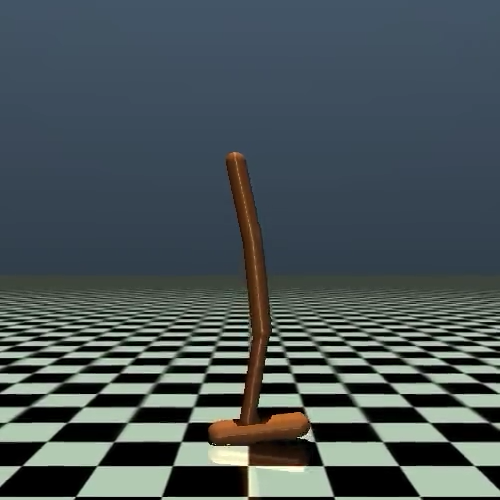
\includegraphics[width=0.2\textwidth]{figures/hopper.png}
        \label{fig:hopper}
    }
    \subcaptionbox{Walker}{
        \centering
        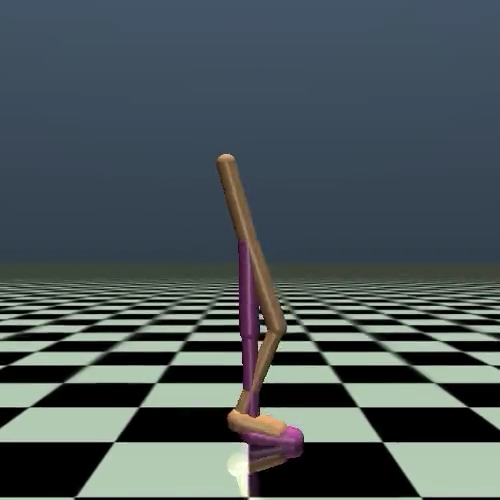
\includegraphics[width=0.2\textwidth]{figures/walker.png}
        \label{fig:walker}
    }
    \subcaptionbox{HalfCheetah}{
        \centering
        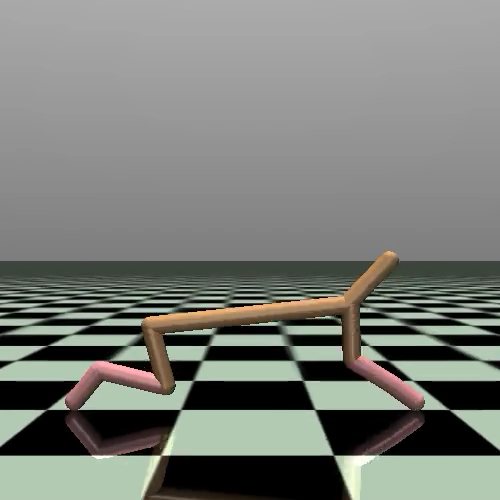
\includegraphics[width=0.2\textwidth]{figures/cheetah.png}
        \label{fig:cheetah}
    }
    \subcaptionbox{Ant}{
        \centering
        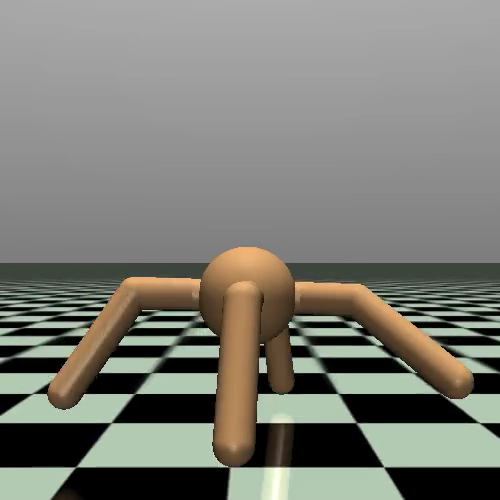
\includegraphics[width=0.2\textwidth]{figures/ant.png}
        \label{fig:ant}
    }
    \caption{实验所使用的四种仿真Mujoco环境示意图}
    \label{fig:env-figures}
\end{figure}

本次实验所使用的参数如表~\ref{tab:hyperparameters}所示进行设定。

\begin{table}
\centering

\begin{tabular}{c|cccccccccc}
\toprule[2pt]
\begin{tabular}[c]{@{}c@{}}environment\\ name\end{tabular} &
  epochs &
  \begin{tabular}[c]{@{}c@{}}env steps\\ per epoch\end{tabular} &
  \begin{tabular}[c]{@{}c@{}}rollout\\ batch\end{tabular} &
  \begin{tabular}[c]{@{}c@{}}policy update\\ per env step\end{tabular} &
  \begin{tabular}[c]{@{}c@{}}model update\\ per env step\end{tabular} &
  $\alpha$ &
  $\beta$ &
  $\gamma$ &
  \begin{tabular}[c]{@{}c@{}}ensemble\\ size\end{tabular} &
  \begin{tabular}[c]{@{}c@{}}network\\ arch\end{tabular} \\
\midrule[1pt]
Hopper      & 120 & 1000 & $10^5$ & 20 & 250 & 0.2 & 0.2 & 0.99 & 10 & \begin{tabular}[c]{@{}c@{}}MLP \\ ($4\times 200$)\end{tabular} \\
Walker2d    & 300 & 1000 & $10^5$ & 20 & 250 & 0.2 & 0.2 & 0.99 & 10 & \begin{tabular}[c]{@{}c@{}}MLP \\ ($4\times 200$)\end{tabular} \\
HalfCheetah & 400 & 1000 & $10^5$ & 40 & 250 & 0.2 & 0.2 & 0.99 & 10 & \begin{tabular}[c]{@{}c@{}}MLP \\ ($4\times 200$)\end{tabular} \\
Ant         & 300 & 1000 & $10^5$ & 20 & 250 & 0.2 & 0.2 & 0.99 & 10 & \begin{tabular}[c]{@{}c@{}}MLP \\ ($4\times 200$)
\end{tabular} \\
\bottomrule[2pt]
\end{tabular}
\caption{MBDP算法验证实验所使用的参数设定}
\label{tab:hyperparameters}

\end{table}

本次实验所使用的代码运行在一台56核CPU、8卡GPU服务器上,具体设备配置如表~\ref{tab:computing-resources}所示。每项任务在计算机上的计算时间如表~\ref{tab:run-time}所示。

\begin{table}
\centering
\begin{tabular}{c|c|c}
\toprule[2pt]
CPU                      & GPU                         & RAM   \\
\midrule[1pt]
Intel E5-2680@2.4GHz (56 Cores) & Tesla P40 (24GB) $\times$ 8 & 256GB\\
\bottomrule[2pt]
\end{tabular}
\caption{MBDP算法验证实验所使用的计算资源}
\label{tab:computing-resources}
\end{table}

\begin{table}
\centering
\begin{tabular}{c|c|c|c|c}
\toprule[2pt]
Environment Name  & Hopper      & Walker2d    & HalfCheetah & Ant         \\
\midrule[1pt]
Time & $\approx 10$ hours & $\approx 20$ hours & $\approx 32$ hours & $\approx 48$ hours \\
\bottomrule[2pt]
\end{tabular}
\caption{单次实验在各环境上的计算时间}
\label{tab:run-time}
\end{table}

\subsection{实验设计与结果分析}

为了证明MBDP方法中上述所加入的模拟数据筛选模块和模型集成筛选模块作为改进方案的可行性,以及验证改进效果,本次实验主要目标为通过实验验证以下问题:

\begin{itemize}
    \item 改进后的算法在强化学习的标准测试任务上相比最新的算法提升如何?
    \item 是否能达到\ref{sec:rollout-method}节中所描述的可以通过动态调整参数$\alpha,\beta$来取得不同决策策略的效果?
\end{itemize}

在四组不同的Mujoco任务上,与最新的MBPO \cite{janner2019trust}算法、STEVE \cite{buckman2018sample}算法、SLBO \cite{Luo2019AlgorithmicGuarantees}算法以及无模型的SAC \cite{haarnoja2018soft}算法进行对比实验。在本课题的算法中,使用了参数$\alpha=0.2, \beta=0.2$。

对比实验结果如图\ref{fig:performance}所示,其中横轴为训练的步数,纵轴为相应步数对应的平均收益。图中实线为不同随机种子实验的均值结果,阴影区域则表示这些实验的方差。由于SAC是无模型强化学习算法,相较基于模型的强化学习算法收敛速度较慢,因此只在图中画出部分训练曲线图,其最终收敛值通过虚线标注出来。

根据实验结果可以看出,本课题设计的改进算法在四种不同的任务环境中,均有着超越现有算法的表现。

\begin{figure}
  \centering
  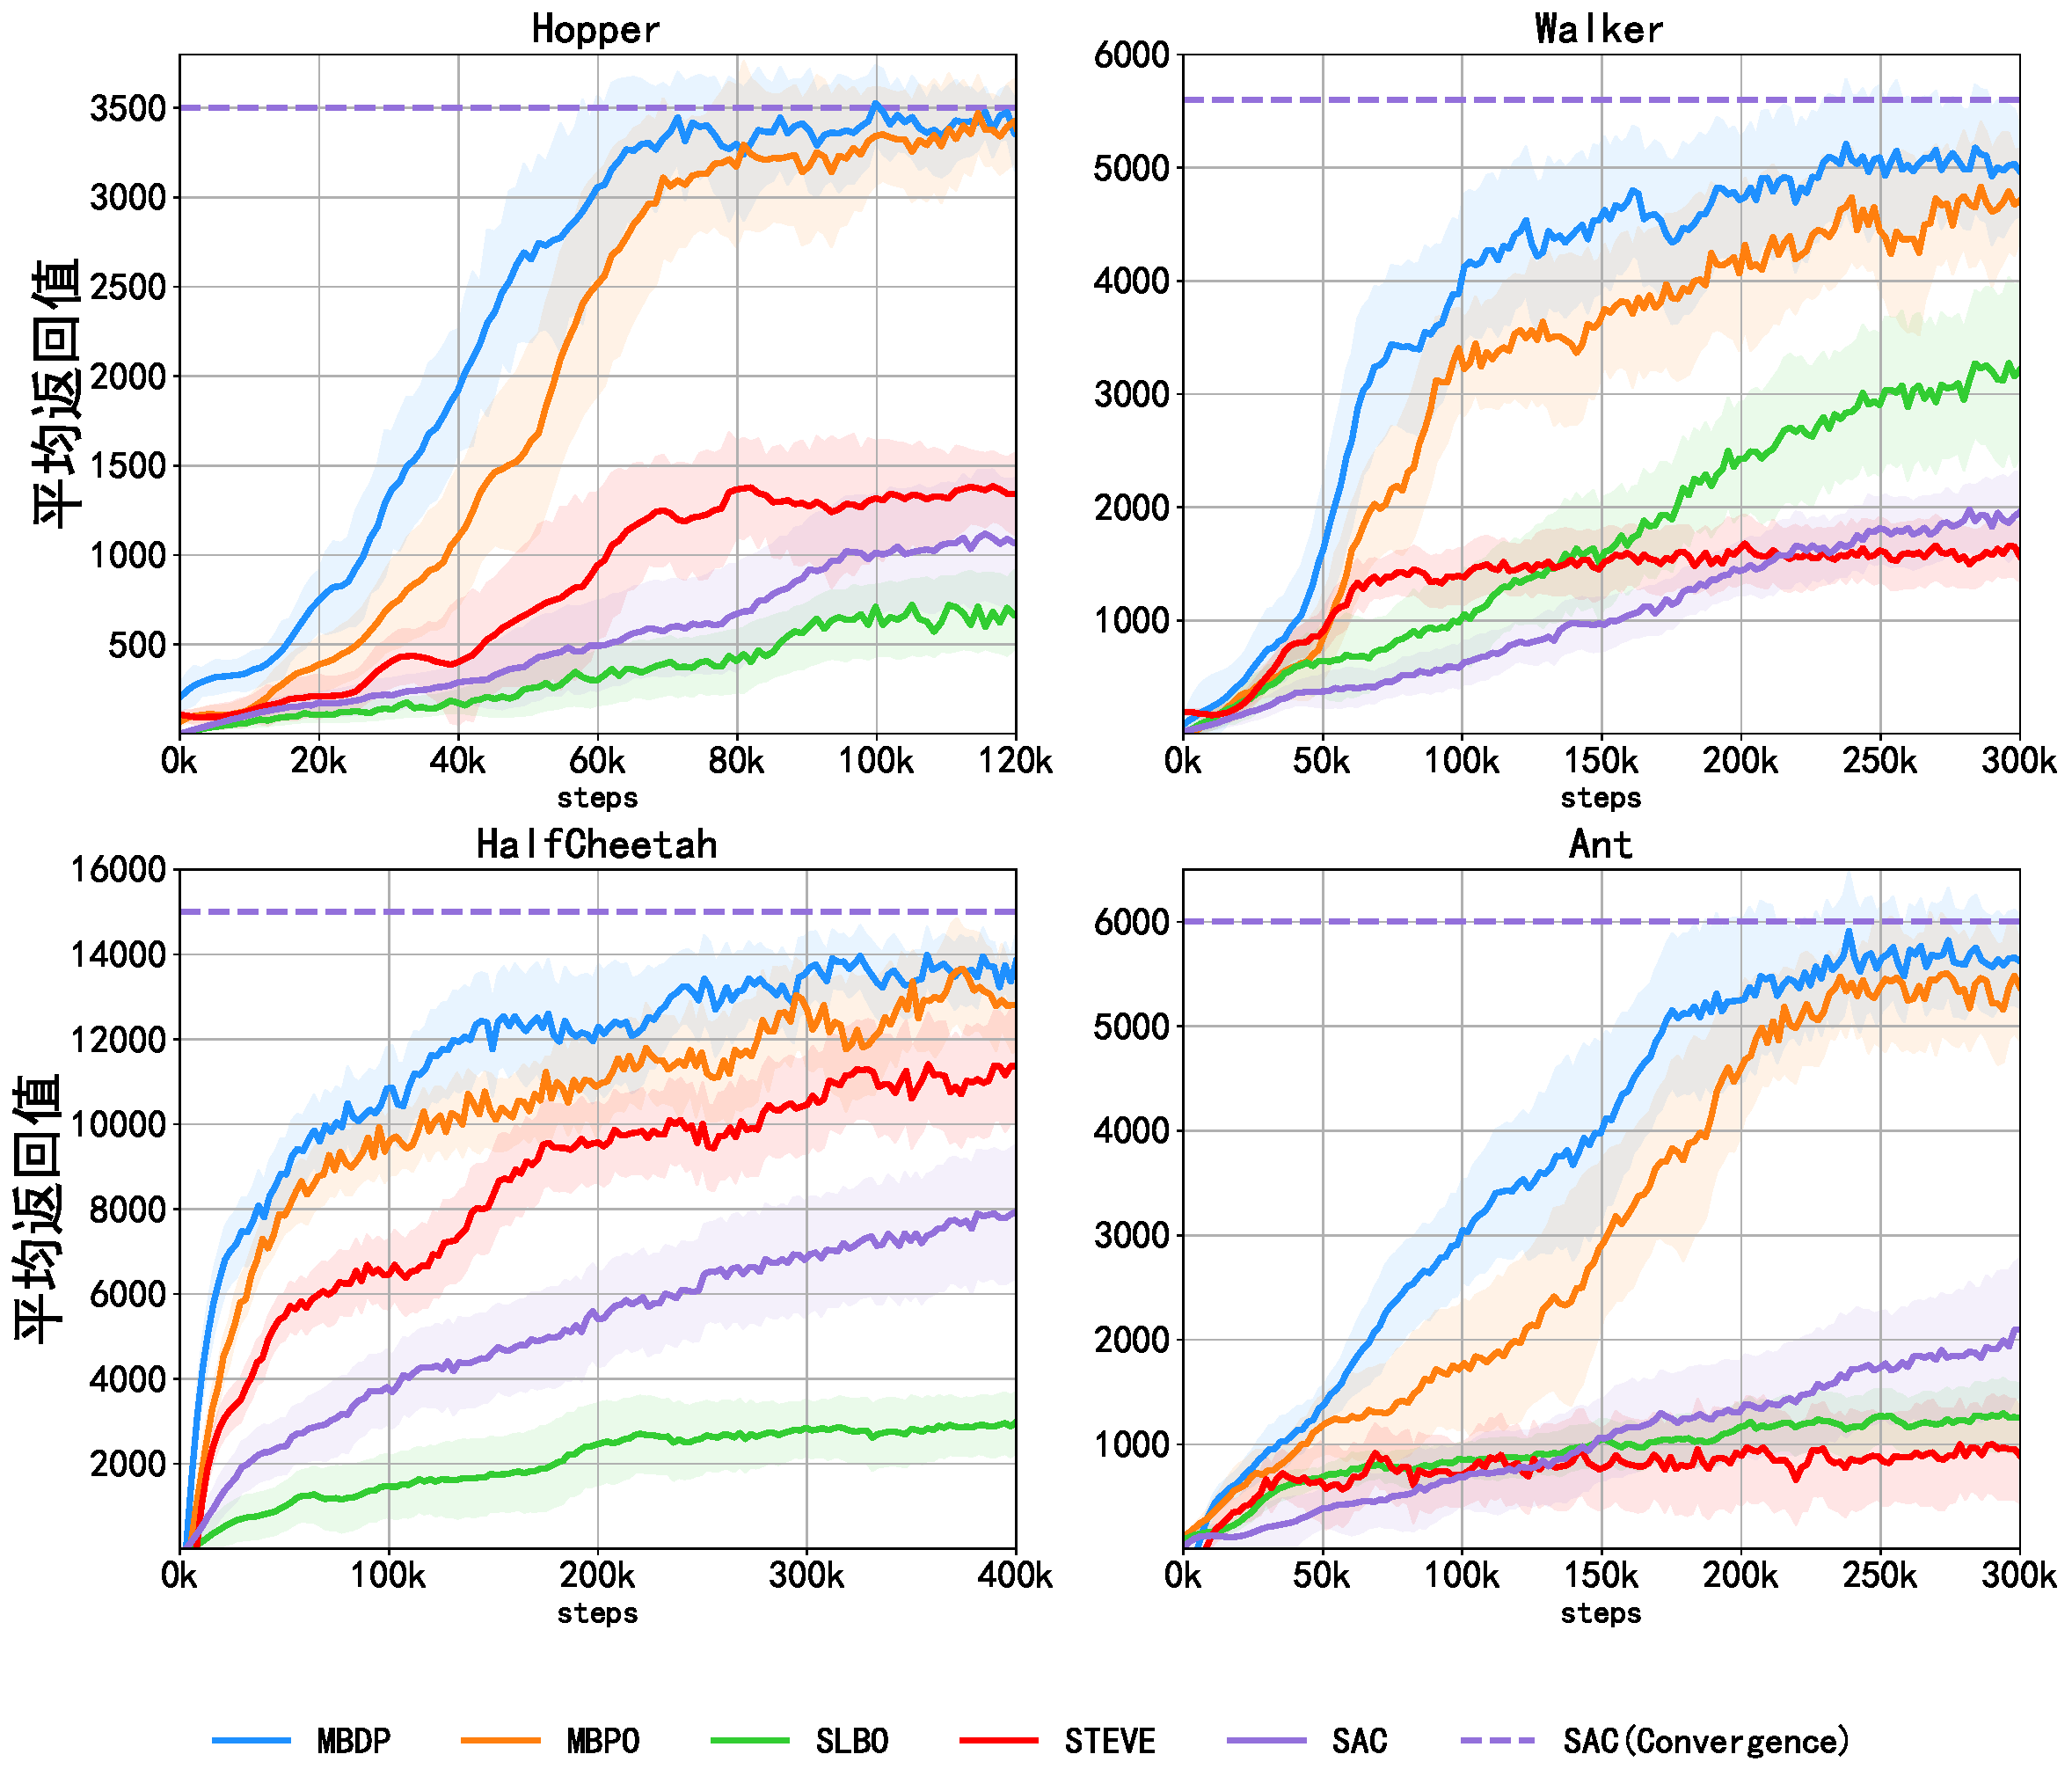
\includegraphics[width=\textwidth]{figures/performance.pdf}
  \caption{各算法在不同任务下的训练曲线图。}
  \label{fig:performance}
\end{figure}

为了进一步验证改进算法的鲁棒性提升,对实验环境加入了不同程度的干扰,本课题在Hopper和HalfCheetah两个任务环境下,将物体的质量和摩擦系数均加以数值区间为$[0.5,1.5]$的干扰,同时以最新的MBPO算法作为对照标准进行对比实验。在各组干扰条件下均进行了一组实验,Hopper任务中每组实验训练$3\times 10^5$轮,HalfCheetah任务中每组任务训练$6\times 10^5$轮,实验结果以热力图的形式绘制成图\ref{fig:robustness-heatmap},其中每一个方格表示一组干扰系数下训练相应轮数后的收益值。观察实验结果可以看出,两种算法尽管在中间的正常区域有着接近的收益,但在干扰较大的环境中,作为对照的MBPO算法并不能有效地学习出决策策略,相比之下本课题的算法则能够较好地处理受干扰较大的环境,这一实验验证了本课题中设计的双筛选机制能够有效提升算法鲁棒性的结论。

\begin{figure}
  \centering
  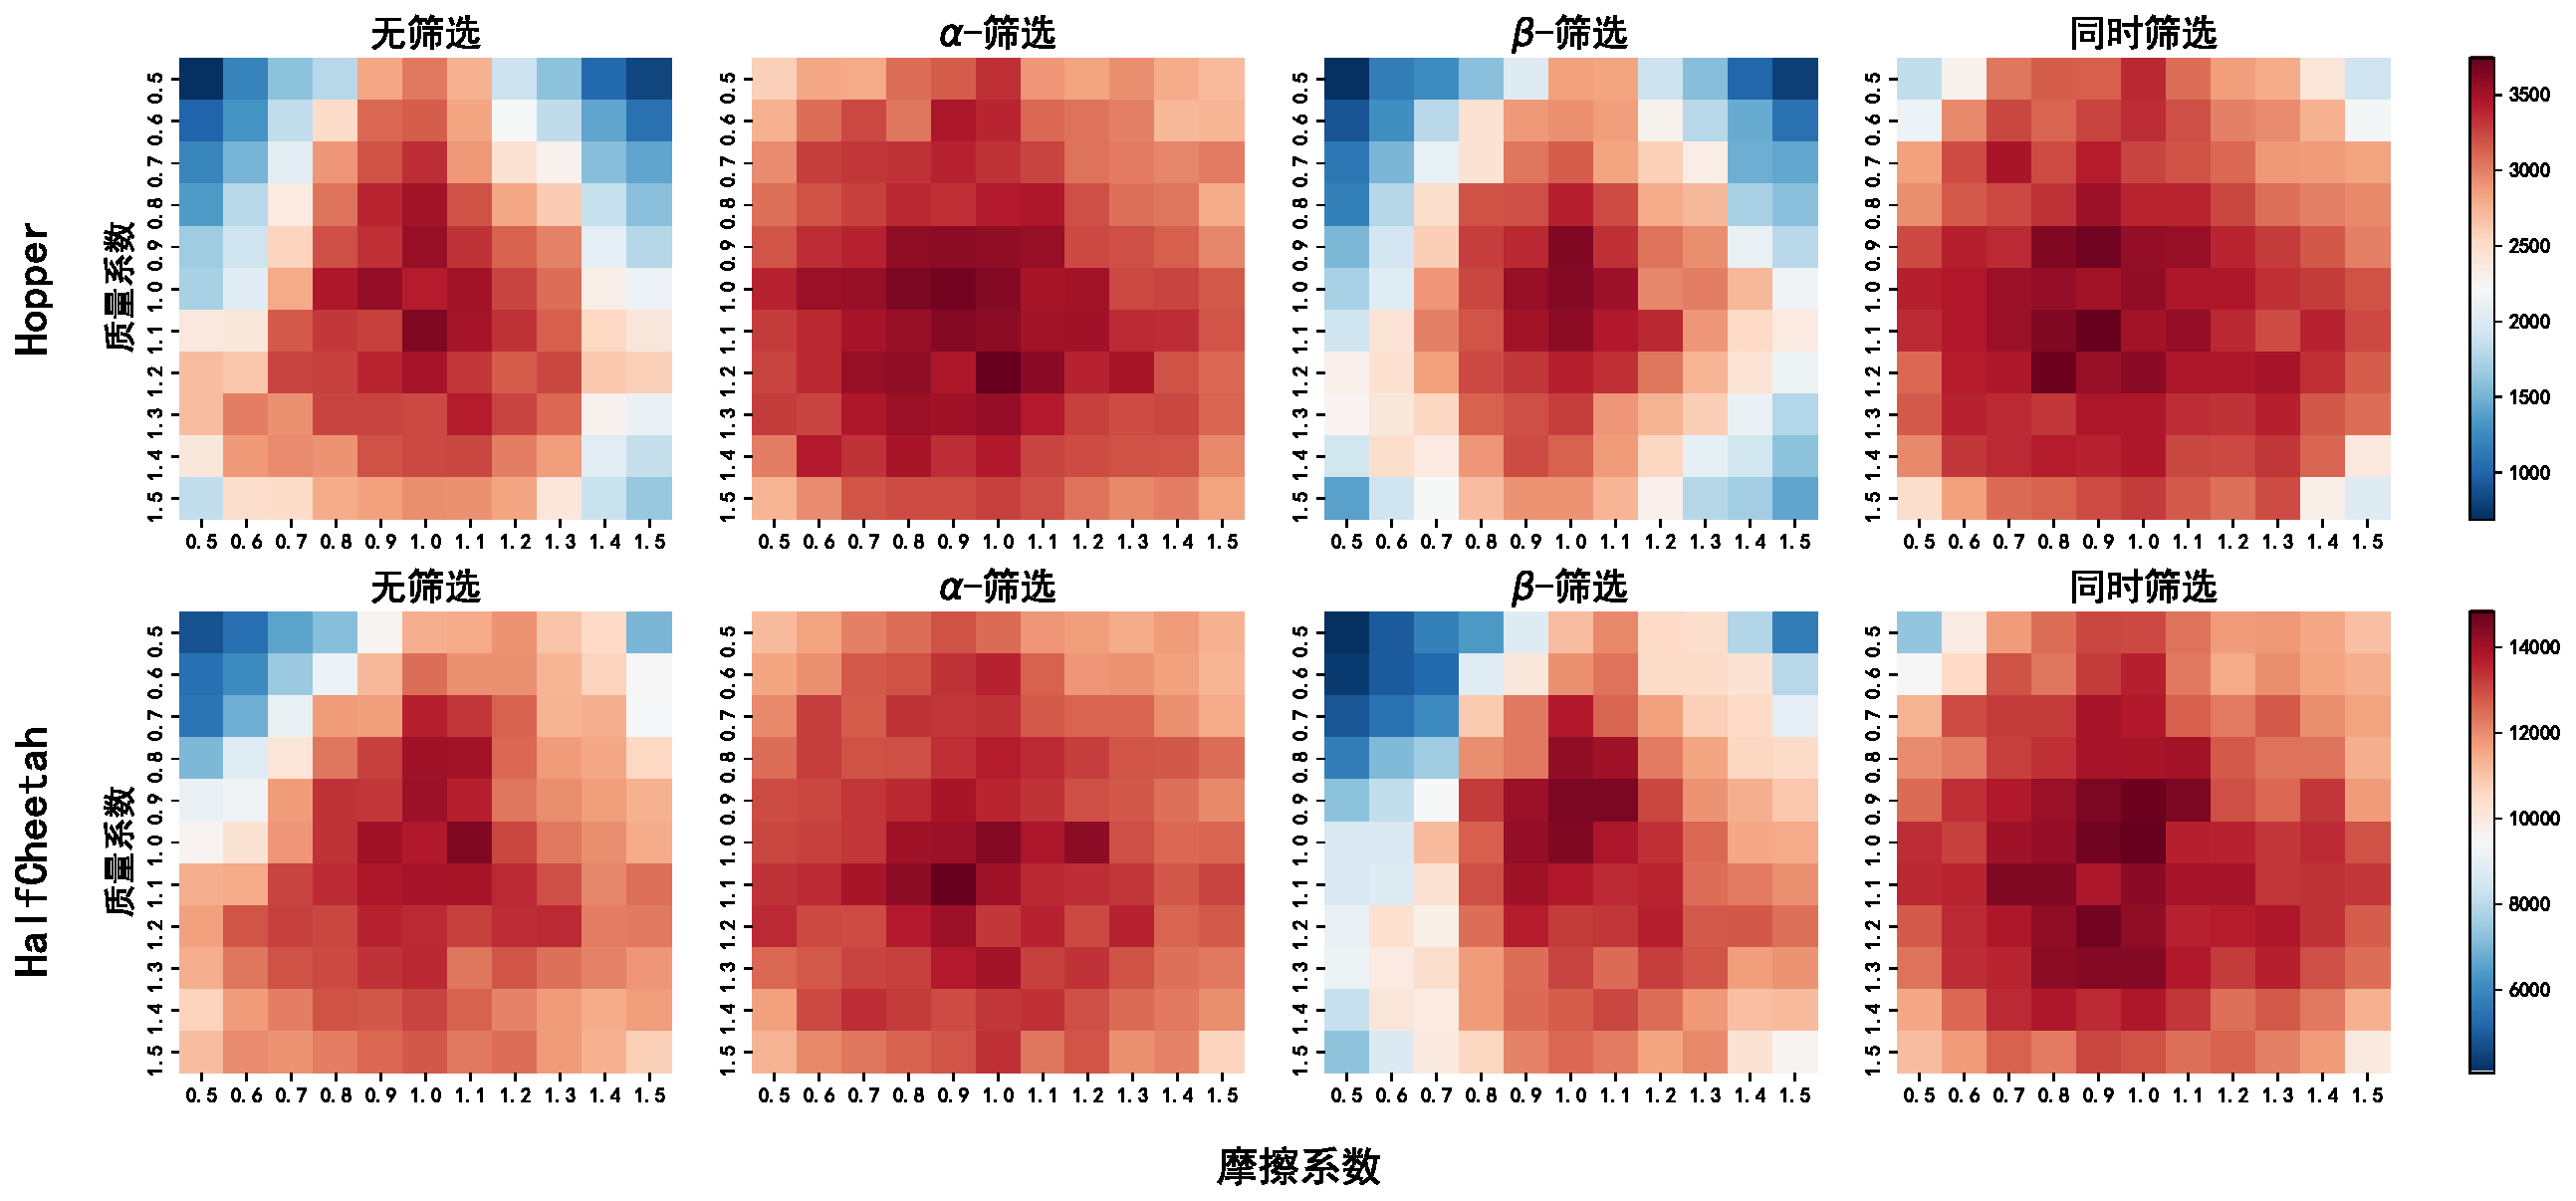
\includegraphics[width=\textwidth]{figures/robustness-heatmap.pdf}
  \caption{算法鲁棒性对比实验。}
  \label{fig:robustness-heatmap}
\end{figure}